\chapter{Wykorzystane technologie}

\section{WebRTC}

\cite{hpbn}

WebRTC jest standardem zapewniającym przeglądarkom możliwości komunikacji peer-to-peer w czasie
rzeczywistym, dzięki czemu możliwe jest budowanie komunikatorów internetowych w całości w obrębie
zapewnianego przez przeglądarkę javascriptowego API. Aby funkcjonalność ta była możliwa do
zrealizowania, niezbędne było użycie wielu protokołów sieciowych, które pokazano na rysunku
\ref{fig:webrtc_stack}.

\begin{figure}[htbp]
    \centering
    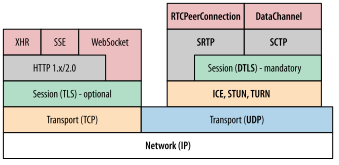
\includegraphics{img/webrtc-stack_hpbn}
    \caption{Stos protokołów w WebRTC - wzięty z HPBN - do zmiany}
    \label{fig:webrtc_stack}
\end{figure}

Głównym targetem WebRTC są przeglądarki, jednak istnieją także implementacje dla innych typów
aplikacji. W podrozdziale \ref{gstreamer_webrtc} opisano implementację dla frameworka GStreamer.

WebRTC pomaga rozwiązać 3 problemy niezbędne do nawiązania multimedialnego połączenia peer-to-peer:

\begin{enumerate}
    \item W jaki sposób zasygnalizować peerowi chęć nawiązania połączenia tak by zaczął on
          nasłuchiwać na wysyłane do niego dane?
    \item Jak wynegocjować odpowiednie parametry strumieni multimedialnych tak by odpowiadały one
          obu stronom?
    \item Jak zidentyfikować potencjalne trasy/tryby połączenia dla obu jego stron?
\end{enumerate}

\subsection{Sygnalizacja nawiązania połączenia}

Before any connectivity checks or session negotiation can occur, we must find out if the other peer
is reachable and if it is willing to establish the connection. We must extend an offer, and the peer
must return an answer (Figure 18-5). However, now we have a dilemma: if the other peer is not
listening for incoming packets, how do we notify it of our intent? At a minimum, we need a shared
signaling channel.

\begin{figure}[H]
    \centering
    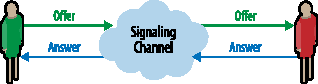
\includegraphics{img/signaling-1}
    \caption{Strony sygnalizacji - wzięty z HPBN - do zmiany}
    \label{fig:signaling}
\end{figure}

WebRTC defers the choice of signaling transport and protocol to the application; the standard
intentionally does not provide any recommendations or implementation for the signaling stack. Why?
This allows interoperability with a variety of other signaling protocols powering existing
communications infrastructure.

W wypadku naszej aplikacji, rola kanału sygnalizacyjnego będzie pełniona przez serwer aplikacji.

\subsection{Negocjacja parametrów połączenia}
\label{negotiation}

WebRTC uses Session Description Protocol (SDP) to describe the parameters of the peer-to-peer
connection. SDP does not deliver any media itself; instead it is used to describe the "session
profile," which represents a list of properties of the connection: types of media to be exchanged
(audio, video, and application data), network transports, used codecs and their settings, bandwidth
information, and other metadata.

To establish a peer-to-peer connection, both peers must follow a symmetric workflow (rysunek
\ref{fig:signaling2}) to exchange SDP descriptions of their respective audio, video, and other data
streams.

\begin{figure}[H]
    \centering
    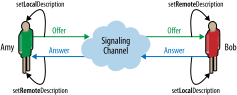
\includegraphics{img/signaling-2}
    \caption{Proces negocjacji - wzięty z HPBN - do zmiany}
    \label{fig:signaling2}
\end{figure}

\begin{enumerate}

    \item The initiator (Amy) registers one or more streams with her local RTCPeerConnection object,
          creates an offer, and sets it as her "local description" of the session.
    \item Amy then sends the generated session offer to the other peer (Bob).
    \item Once the offer is received by Bob, he sets Amy's description as the "remote description"
          of the session, registers his own streams with his own RTCPeerConnection object, generates
          the "answer" SDP description, and sets it as the "local description" of the session—phew!
    \item Bob then sends the generated session answer back to Amy.
    \item Once Bob's SDP answer is received by Amy, she sets his answer as the "remote description"
          of her original session.
\end{enumerate}

With that, once the SDP session descriptions have been exchanged via the signaling channel, both
parties have now negotiated the type of streams to be exchanged, and their settings. We are almost
ready to begin our peer-to-peer communication! Now, there is just one more detail to take care of:
connectivity checks and NAT traversal.

\subsection{Interactive Connectivity Establishment (ICE)}
\label{ice}

In order to establish a peer-to-peer connection, by definition, the peers must be able to route
packets to each other. A trivial statement on the surface, but hard to achieve in practice due to
the numerous layers of firewalls and NAT devices between most peers.

First, let's consider the trivial case, where both peers are located on the same internal network,
and there are no firewalls or NATs between them. To establish the connection, each peer can simply
query its operating system for its IP address (or multiple, if there are multiple network
interfaces), append the provided IP and port tuples to the generated SDP strings, and forward it to
the other peer. Once the SDP exchange is complete, both peers can initiate a direct peer-to-peer
connection.

So far, so good. However, what would happen if one or both of the peers were on distinct private
networks? We could repeat the preceding workflow, discover and embed the private IP addresses of
each peer, but the peer-to-peer connections would obviously fail! What we need is a public routing
path between the peers. Thankfully, the WebRTC framework manages most of this complexity on our
behalf:

\begin{itemize}
    \item Each RTCPeerConnection connection object contains an "ICE agent."
    \item ICE agent is responsible for gathering local IP, port tuples (candidates).
    \item ICE agent is responsible for performing connectivity checks between peers.
    \item ICE agent is responsible for sending connection keepalives.
\end{itemize}

Once a session description (local or remote) is set, local ICE agent automatically begins the
process of discovering all the possible candidate IP, port tuples for the local peer:

\begin{enumerate}
    \item ICE agent queries the operating system for local IP addresses.
    \item If configured, ICE agent queries an external STUN server to retrieve the public IP and
          port tuple of the peer.
    \item If configured, ICE agent appends the TURN server as a last resort candidate. If the
          peer-to-peer connection fails, the data will be relayed through the specified
          intermediary.
\end{enumerate}

As the example illustrates, the ICE agent handles most of the complexity on our behalf: the ICE
gathering process is triggered automatically, STUN lookups are performed in the background, and the
discovered candidates are registered with the RTCPeerConnection object. Once the process is
complete, we can generate the SDP offer and use the signaling channel to deliver it to the other
peer.

\section{GStreamer}

GStreamer jest frameworkiem do tworzenia strumieniujących aplikacji multimedialnych
\cite{gstreamer}. Aplikacje są wyrażane jako "rurociąg" składający się z bloków. Rdzeń GStreamer
definiuje architekturę aplikacji oraz API dla elementów, a same elementy są zawarte w różnych
pluginach. Jego modularna architektura sprawia że nie jest ograniczony do aplikacji audio-wideo,
lecz może być wykorzystany do każdej aplikacji, która strumieniowo przetwarza dowolne rodzaje
danych.

\begin{figure}[H]
    \centering
    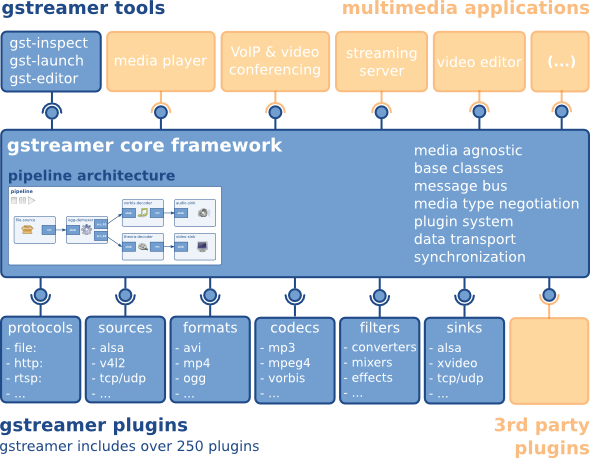
\includegraphics[width=.5\textwidth]{img/technologie/gstreamer-overview}
    \caption{Architektura projektu GStreamer}
\end{figure}

Dane generowane są elementach-źródłach (source), są przetwarzane przez elementy-filtry (filter), a
następnie są konsumowane w elementach-zlewach (sinks). Elementy są częścią rurociągu, który w danym
czasie może być zatrzymany, zapauzowany, lub uruchomiony. Zmiana stanu rurociągu zmienia stan
wszystkich jego elementów.

\begin{figure}[H]
    \centering
    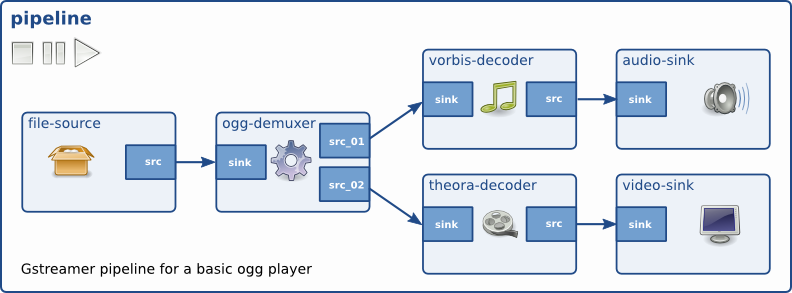
\includegraphics[width=.7\textwidth]{img/technologie/simple-player}
    \caption{Przykładowy rurociąg aplikacji GStreamer}
    \label{fig:gstreamer_example_pipeline}
\end{figure}

Rysunek \ref{fig:gstreamer_example_pipeline} przedstawia rurociąg przykładowego odtwarzacza plików
OGG. Dane przechodzą przez rurociąg od lewej do prawej strony, będąc transformowane w każdym
elemencie.

\subsection{GStreamer WebRTC}
\label{gstreamer_webrtc}

GStreamer posiada swoją własną implementację WebRTC, wykonaną przez firmę Centricular. Jej głównym
elementem jest element
\href{https://gstreamer.freedesktop.org/documentation/webrtc/index.html?gi-language=c}{webrtcbin}.
Ten element zajmuje się procesami negocjacji parametrów połączenia oraz zbierania i udostępniania
kandydatów ICE omówionymi w podrozdziałach \ref{negotiation} i \ref{ice}. Zdarzenia takie jak
pojawienie się nowego strumienia multimedialnego są komunikowane aplikacji za pomocą sygnałów, które
są obsługiwane zazwyczaj poprzez tworzenie nowych elementów i dodanie ich do rurociągu celem
prezentacji przychodzącego strumienia użytkownikowi.

\section{GTK4 i libadwaita}

Do wykonania aplikacji graficznej wykorzystany został darmowy, otwartoźródłowy, wieloplatformowy
framework GTK4 oraz biblioteka libadwaita implementująca często wykorzystywane komponenty i wzorce
projektowe będące częścią wytycznych projektu GNOME w projektowaniu interfejsów
(\href{https://developer.gnome.org/hig/}{GNOME Human Interface Guidelines}).

GTK jest najpopularniejszą biblioteką używaną do tworzenia graficznych aplikacji dla systemów Linux.
Napisana w C, wykorzystuje jednak paradygmat obiektowy; używa biblioteki GObject która zapewnia
system klas i obiektów, a także inne zależności widoczne na rysunku \ref{fig:gtk_toolkit}.

\begin{figure}[H]
    \centering
    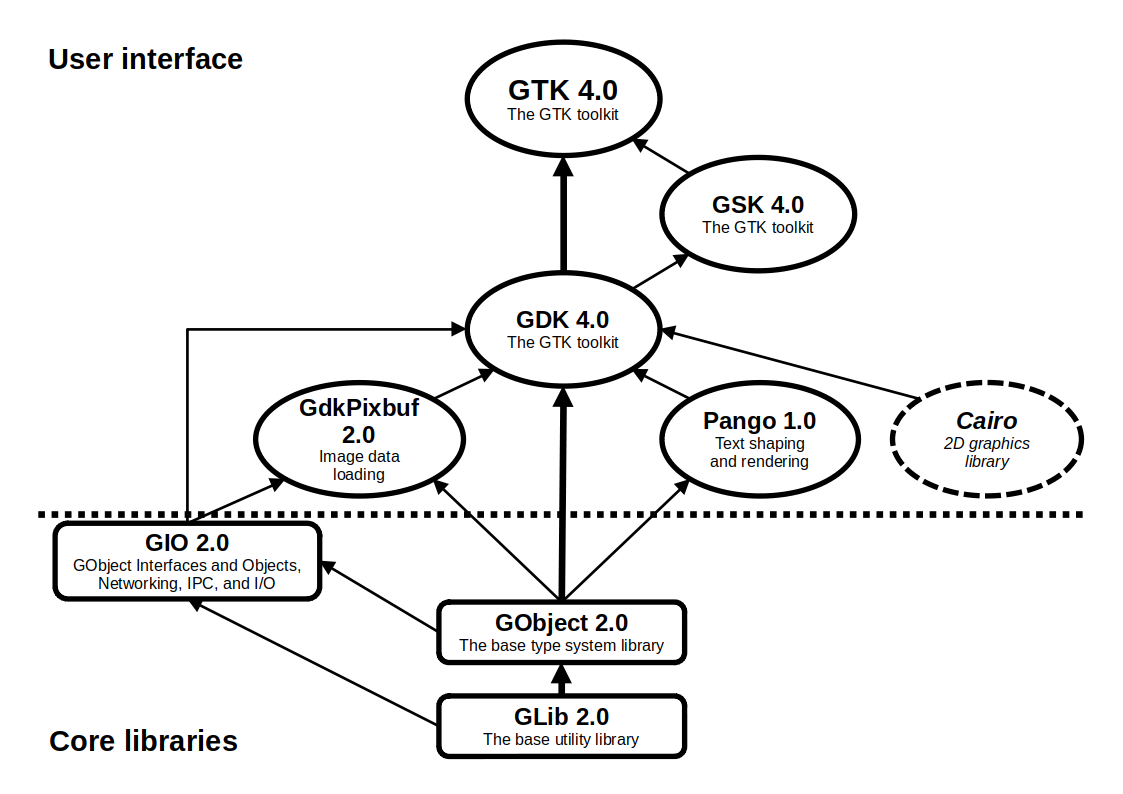
\includegraphics[width=.7\textwidth]{img/gtk-toolkit}
    \caption{Architektura zestawu narzędzi GTK}
    \label{fig:gtk_toolkit}
\end{figure}

Bezpośrednie używanie tych bibliotek w języku Rust nie jest jednak rekomendowane, i gdzie tylko
możliwe wykorzystywane są biblioteki natywne dla języka Rust. Nie można ich jednak wyeliminować lub
zastąpić, ponieważ są twardymi zależnościami frameworka GUI.

Pomimo tego, GTK zostało wybrane z dwóch powodów:

\begin{itemize}
    \item GTK jest najpopularniejszym, najbardziej sprawdzonym oraz dojrzałym frameworkiem GUI dla
          systemów Linux
    \item GStreamer i GTK są częściami tego samego projektu freedesktop i w związku z tym
          interoperują ze sobą; m.in. wykorzystują te same biblioteki GLib i GObject, a także
          GStreamer może rysować zawartość strumienia mediów na powierzchnię jeżeli ta implementuje
          interfejs \verb|GstVideoOverlay|.
\end{itemize}

\section{Rust}

Rust jest językiem programowania generalnego zastosowania rozwijanym przez fundację Mozilla.
Stworzony z myślą o bezpieczeństwie, współbieżności, i praktyczności, zapewnia wydajność bliską
języka C jednocześnie gwarantując bezpieczeństwo pamięci nie wykorzystując przy tym mechanizmu
Garbage Collection. Zamiast tego Rust wykorzystuje "borrow checker", który śledzi czas życia
referencji do obiektów podczas kompilacji. Dzięki temu niektóre klasy błędów są niemożliwe do
popełnienia, dzięki czemu programista może wykorzystywać wielowątkowość bez obaw przed ezoterycznymi
i nietrywialnymi do zdebugowania błędami typu race-condition. Ponadto dzięki darmowym abstrakcjom,
kod w języku Rust jest czytelny jak język wysokopoziomowy, jednocześnie zapewniając wydajność
charakterystyczną zazwyczaj tylko dla języków niskopoziomowych.

\section{Programowanie asynchroniczne}

Programowanie asynchroniczne jest paradygmatem programowania umożliwiającym konkurentne wykonywanie
wielu zadań bez użycia mechanizmów wielowątkowości. Zamiast tego, główny wątek programu może zapisać
stan aktualnie wykonywanego zadania i zająć się wykonywaniem innego zadania. Paradygmat ten
jest popularny przy programowaniu serwerów, ponieważ wielowątkowość charakteryzowała się wieloma
wadami:

\begin{itemize}
    \item Wątki są powolne do tworzenia, i zajmują pewną minimalną ilość pamięci - zadania
          asynchroniczne można tworzyć bardzo szybko i zajmują one o wiele mniej pamięci
    \item Użycie wielu wątków może prowadzić do błędów typu race-condition - zadania asynchroniczne
          mogą być przypisane do jednego wątku eliminując ten problem
    \item Jeżeli używana jest bardzo duża liczba wątków, overhead systemu operacyjnego staje się
          znaczący i wydajność systemu może ucierpieć - w systemie asynchronicznym planowanie zadań
          jest prostsze ponieważ dzieje się w userspace przez egzekutor systemu asynchronicznego,
          nie występują zatem drogie context-switche, a także egzekutor lepiej zna charakterystyki
          wykonywanego kodu więc może planować tak by zużycie zasobów było mniejsze
    \item Większość sytuacji wymagających konkurentności w serwerach to czekanie na jakieś
          zdarzenie: czekanie na połączenie, czekanie na odebranie danych od klienta, etc. tzw.
          IO-bound. W takiej sytuacji nie ma potrzeby zwiększać złożoności systemu angażując kolejne
          fizyczne procesory i pamięć, zamiast tego wątek może w tym czasie pracować nad innymi
          zadaniami.
\end{itemize}

Ekosystem programowania asynchronicznego składa się z asynchronicznych tzw. runtimes zawierających
egzekutory zadań asynchronicznych oraz samych zadań asynchronicznych znanych jako Futures. Future
(ang. przyszłość) reprezentuje operacje która zwróci wartość w przyszłości i musi być w tym celu
możliwie wielokrotnie wykonywana funkcją \verb|poll()|, która może zwrócić wariant
\verb|Poll::Ready(T)| reprezentujący zakończenie działania i zwrócenie wartości, lub wariant
\verb|Poll::Pending| wskazujący że wykonany został pewien postęp w wykonaniu, jednak funkcja będzie
musiała zostać wykonana ponownie.

Sam egzekutor wykorzystuje asynchroniczne system calle takie jak epoll, które sprawiają że gdy
wydarzy się zdarzenie, w kontekście future wywołuje się funkcja \verb|wake()|, która powiadamia
egzekutor o tym że dana future może być pollnięta ponownie.

Overhead takiego podejścia jest mały i działa ono bardzo dobrze, dopóki futures są IO-bound, tj.
większość czasu to czas spędzony na czekanie na IO. Gdy futures są CPU-bound, tj. wykonują dużą
ilość kalkulacji których zakończenie zajmie znaczącą ilość czasu (np. kilka sekund), lub używają
synchronicznych blokujących API, wtedy taka future jest w stanie zablokować egzekutor i inne futures
nie będą w stanie się wykonać. W tym celu asynchroniczne runtimes zazwyczaj udostępniają specjalny
thread pool na zadania blokujące główny wątek. Dodatkowo, egzekutor zazwyczaj też wykorzystuje
threadpool do uruchamiania futures, dzięki czemu mogą być one wykonywane nie tylko konkurentnie lecz
także równolegle. Dzięki gwarancjom bezpieczeństwa i systemowi ownership w języku Rust, nie powoduje
to ryzyka wystąpienia błędów związanych z wielowątkowością. To czy future może zostać wysłana
pomiędzy wątkami jest wiadome już w procesie kompilacji, dzięki traitowi \verb|Send|. Funkcje
egzekutorów typu \verb|task::spawn()| służące do rozpoczęcia konkurentnego wykonania danego future
wymagają aby była ona \verb|Send|, a jeżeli nie jest, emitowany jest błąd kompilacji. Istnieją także
funkcje jak \verb|task::block_on()| które synchronicznie wykonują dany future na jednym wątku.

W niniejszym projekcie gdy tylko możliwe preferowane jest używanie asynchronicznych API.
Wykorzystywane są oba najpopularniejsze runtime'y asynchroniczne w języku Rust: tokio oraz
async-std.

